\documentclass[a4paper,11pt]{article}
%\usepackage[slovene]{babel}
\usepackage[utf8]{inputenc}
\usepackage[T1]{fontenc}

\usepackage{graphicx}
\usepackage{tabularx}
\usepackage{url}

\newcolumntype{Y}{>{\centering\arraybackslash}X}

\begin{document}
\thispagestyle{empty}
%\setlength{\parindent}{0em}


\includegraphics[scale=0.35]{UUlogo.png}

\vspace{50mm}

\begin{center}
\begin{large}
Data Mining: Assignment 1 \\[3mm]
\textbf{
\uppercase{Classification Trees, Bagging and Random Forests}} \\[25mm]
\end{large}

\begin{tabularx}{\textwidth}{YY}
Ana Borovac & Argyro (Iro) Sfoungari \\
6584446 & 6528015
\end{tabularx}
\end{center}

\vfill

October, 2018

\newpage

\tableofcontents

\begin{abstract}
    In the first Data Mining assignment, we were asked to write two main functions tree.grow and tree.classify with specific input arguments each. Initially, we had to create a single tree, but then we had to expand it to Bagging and Random Forests by adding two auxiliary functions, tree.grow.bag and tree.classify.bag. The above code was created in order to analyse the Eclipse Bug Dataset. More specifically we had to do some tests in order to predict if any post release bugs have been reported. In other words, we created a single tree for both the training and the test set, while at the same time we followed the same procedure for Bagging and Random Forests. Finally, we examined accuracy, precision and recall for each dataset and case and we ended up to the following conclusion. With $Z$-test we proved that the difference in the classification accuracy between Single Tree and Random Forests is not statistically significant, otherwise it is. 
    
We ran the code several times to check our results and although there were some small differences, we chose to present the most representative.
\end{abstract}

\section{Short Description of the Data}
  In the assignment we are asked to use the algorithms we have implemented to analyse the bug dataset of the Eclipse programming environment, before and after the release of each packet. According to the accompanying article \cite{article}, in order to explain the reason why some programs are more vulnerable to failure than others, we need to take a look at a bug database. Bug databases, list all the errors that occurred during the lifetime of a software. More specifically, the dataset contains information about the number of faults that have been reported in the first six months before and after release. As reported by the authors, metrics are useful for predicting the thickness of the defects. For the assignment we are going to use the 2.0 release as the training set and the 3.0 release as the test set and we are going to monitor if errors have been reported to later versions. We are asked to use the same metrics as the authors and the number of pre-release bugs. 
 
 These metrics are: 
 \begin{itemize}
 \item FOUT      (Number of method calls) 
 \item MLOC     (Method lines of code)
 \item NBD        (Nested block depth)
 \item PAR        (Number of parameters) 
 \item VG          (McCabe cyclomatic complexity)
 \item NOF        (Number of fields)
 \item NOM       (Number of methods) 
 \item NSF        (Number of static fields)
 \item NSM       (Number of static methods)
 \item ACD       (Number of anonymous type declarations)
 \item NOI        (Number of interfaces)
 \item NOT       (Number of classes)
 \item TLOC     (Total lines of code)
 \item NOCU    (Number of files)
 \end{itemize}
And Pre-released defects: the defects that are observed during the development and testing of a program. 

The training set consists of 377 samples:
\begin{itemize}
\item 187 samples labeled 0
\item 190 samples labeled 1
\end{itemize}

The test set consists of 661 samples:
\begin{itemize}
\item 348 samples labeled 0
\item 313 samples labeled 1
\end{itemize}

\section{Single Tree}
Below (figure \ref{fig: tree1}) we have reproduced the first few splits of the single tree. We continue splitting until we get the representation of the left sub-tree. We have to process the given data, and draw to some conclusions in order to decide whether our classification rule makes sense. In our tree, the initial split is based on the number of pre-released defects that are detected during the development and testing of the program. As the split begins, we see that for the better case which is the one with the fewest pre-released defects ($\leq 4.5$), we have a shorter cyclomatic complexity (a software metric, used to indicate the complexity of a program) \verb|VG_max|. This split seems quite reasonable if we think that with a more complex code we predict more bugs and vice versa, with fewer pre-released defects the complexity is reduced accordingly. Then, we split into the smaller total number of static methods \verb|NSM_sum|, fewer total number of method calls \verb|FOUT_sum|, smaller average of nested block depth \verb|MBD_avg|, fewer maximum number of fields \verb|NOF_max|, smaller average number of methods \verb|NOM_avg| and static methods \verb|NSM_avg| respectively and finally fewer lines of code. Consequently, we could support that the classification rule we created leads to reasonable results, as less complex code, gives less methods, method calls and other programming structures and finally fewer total lines of code. 

\begin{figure}[h!]
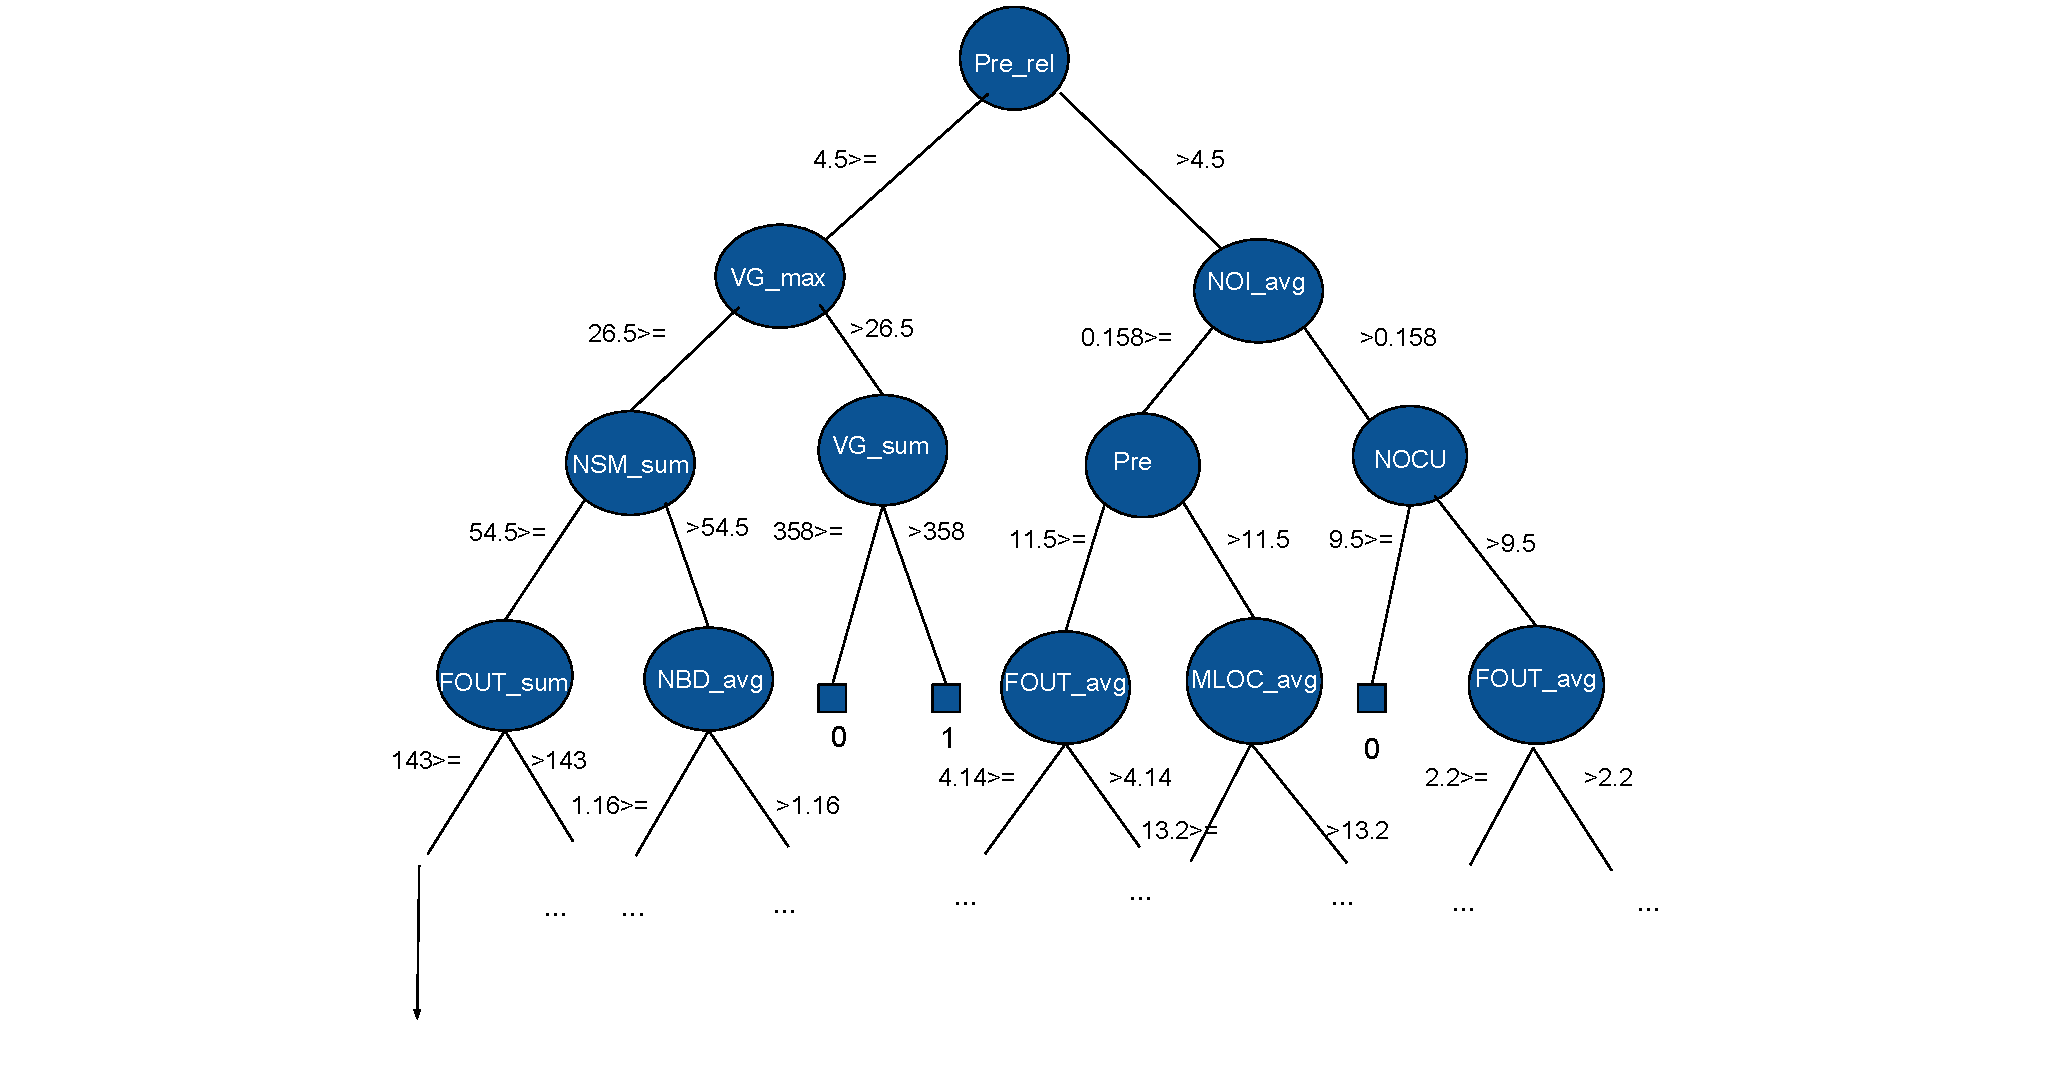
\includegraphics[width=\textwidth]{Tree1.pdf}
\caption{First splits of the trained single tree.}
\label{fig: tree1}
\end{figure}

\begin{figure}[h!]
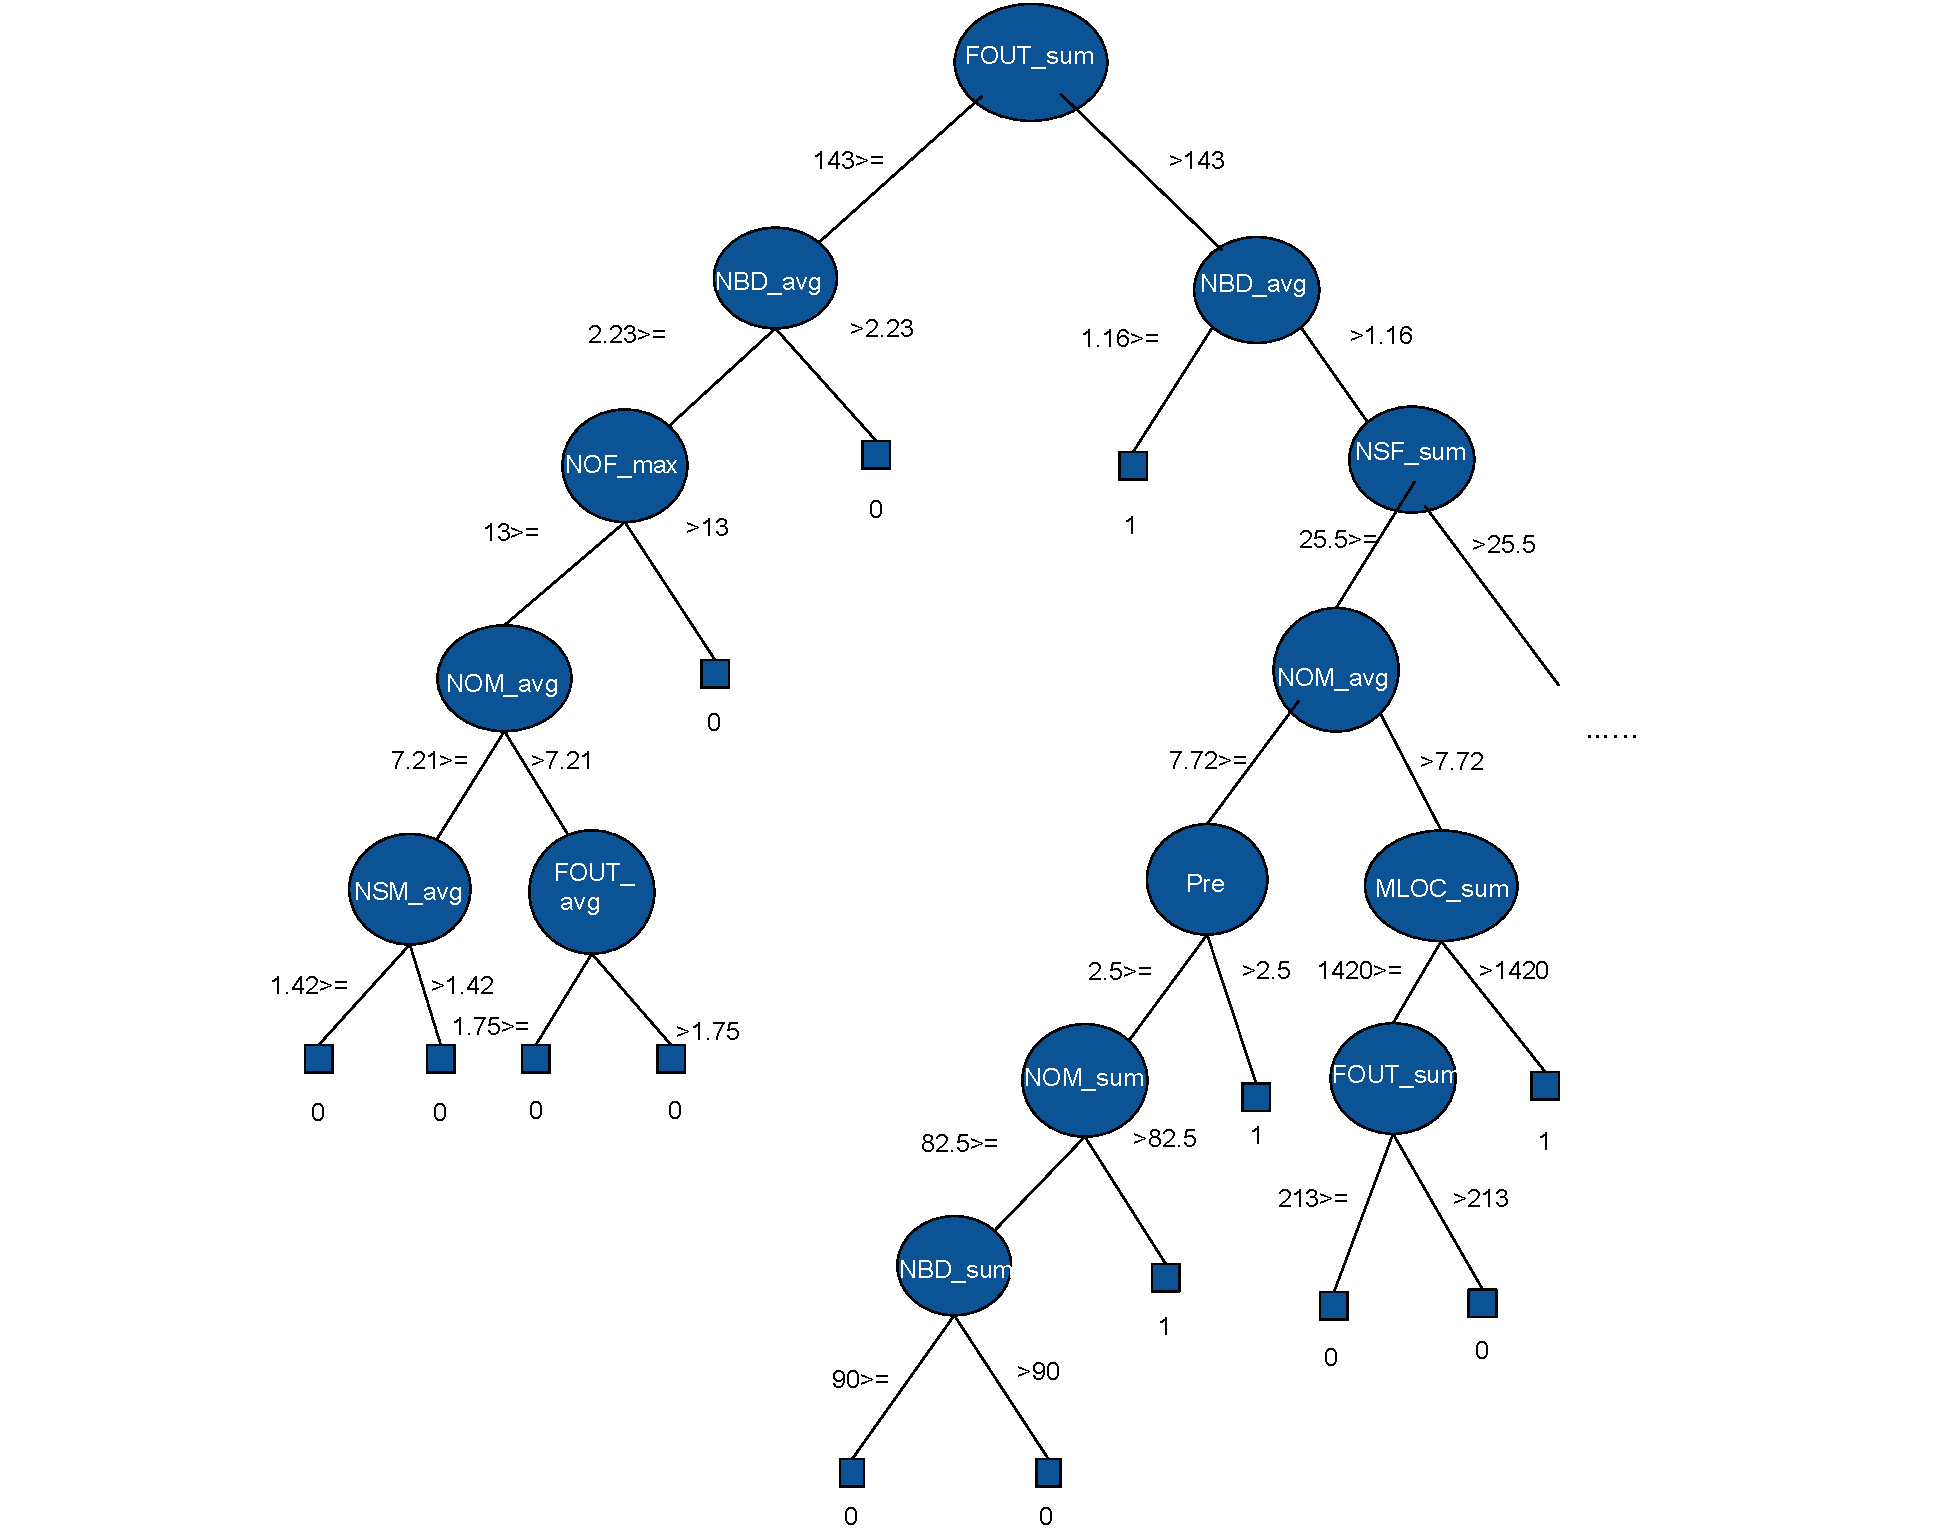
\includegraphics[width=\textwidth]{Tree2.pdf}
\caption{Continuation of the tree from figure \ref{fig: tree1}.} 
\label{fig: tree2}
\end{figure}

\section{Single Tree, Bagging and Random Forests}

\subsection{Single Tree}
We trained a single classification tree on the training set with \verb|nmin = 15|, \verb|minleaf = 5| and \verb|nfeat = 41|. On the test set we got the following confusion matrix \ref{tab: singletree}.
 
\begin{table}[h!]
\centering
	\begin{tabular}{c||c|c}
	True class \textbackslash\ Predicted class & 0 & 1 \\ \hline \hline
	0 & 266 & 82 \\ \hline
	1 & 128 & 185
	\end{tabular}
	\caption{Confusion matrix for a single tree run on the test set.}
	\label{tab: singletree}
\end{table}


\subsection{Bagging}
We used bagging with \verb|nmin = 15|, \verb|minleaf = 5| and \verb|nfeat = 41| and \verb|m = 100|. On the test set we got the following confusion matrix \ref{tab: bagging}.

\begin{table}[h!]
\centering
	\begin{tabular}{c||c|c}
	True class \textbackslash\ Predicted class & 0 & 1 \\ \hline \hline
	0 & 306 & 42 \\ \hline
	1 & 104 & 209
	\end{tabular}
	\caption{Confusion matrix for a bagging run on the test set.}
	\label{tab: bagging}
\end{table}



\subsection{Random Forests}
We used random forests with \verb|nmin = 15|, \verb|minleaf = 5| and  \verb|nfeat = 6|. On the test set we got the following confusion matrix \ref{tab: randomforest}.

\begin{table}[h!]
\centering
	\begin{tabular}{c||c|c}
	True class \textbackslash\ Predicted class & 0 & 1 \\ \hline \hline
	0 & 258 & 90 \\ \hline
	1 & 111 & 202
	\end{tabular}
	\caption{Confusion matrix for a random forests run on the test set.}
	\label{tab: randomforest}
\end{table}



\section{Differences in Accuracy}
First, let's have a look at table the \ref{tab: apr}. We can see that accuracy of Bagging is higher that accuracies of Single Tree and Random Forests. So, in the next step we would like to see if the difference is statistically significant.

\begin{table}[h!]
\centering
	\begin{tabular}{l||c|c|c}
	& Accuracy & Precision & Recall \\ \hline \hline
	Single Tree & 0{,}68 & 0{,}69 & 0{,}59 \\ \hline
	Bagging & 0{,}78 & 0{,}83 & 0{,}67 \\ \hline
	Random Forests & 0{,}70 & 0{,}69 & 0{,}65 
	\end{tabular}
	\caption{Accuracies, precisions and recalls of models: Single Tree, Bagging and Random Forests.}
	\label{tab: apr}
\end{table}

To test if the differences in accuracy found on the test set are statistically significant we used $Z$-test \cite{accuracy}:
\[
Z = \frac{|f_{12} - f_{21}|}{\sqrt{f_{12} + f_{21}}}
\]
where $f_{12}$ denotes the number of samples that were classified correctly by the first algorithm and misclassified by the second algorithm (similar for $f_{21}$). If $Z \geq 1{,}96$ that means that a difference in the classification accuracy between the confusion matrices is statistically significant ($p \leq 0{,}05$).

In the table \ref{tab: z} there are $Z$-values for all the possible comparisons.
\begin{table}[h!]
\centering
	\begin{tabular}{l||c}
	Compared algorithms & $Z$-value   \\ \hline \hline
	Single Tree, Random Forests & 0{,}68 \\ \hline
	Single Tree, Bagging &  5{,}75 \\ \hline
	Bagging, Random Forests & 4{,}57
	\end{tabular}
	\caption{Calculated $Z$-values.}
	\label{tab: z}
\end{table}

We can conclude that the difference in the classification accuracy between the confusion matrices of Single Tree and Random Forests is not statistically significant. In the other two cases, the difference is statistically significant.

\bibliographystyle{plain}
\bibliography{references}

\end{document}










